\documentclass[12pt]{article}
 
\usepackage[margin=1in]{geometry} 
\usepackage{amsmath,amsthm,amssymb}
\usepackage{graphicx}
\usepackage{epstopdf}
 
\newcommand{\N}{\mathbb{N}}
\newcommand{\Z}{\mathbb{Z}}
 
\newenvironment{exercise}[2][Exercise]{\begin{trivlist}
\item[\hskip \labelsep {\bfseries #1}\hskip \labelsep {\bfseries #2.}]}{\end{trivlist}}
\newenvironment{problem}[2][Problem]{\begin{trivlist}
\item[\hskip \labelsep {\bfseries #1}\hskip \labelsep {\bfseries #2.}]}{\end{trivlist}}
 
\usepackage{geometry}
\usepackage{courier}
\usepackage{color}
\usepackage{listings}
\definecolor{dkgreen}{rgb}{0,0.6,0}
\definecolor{gray}{rgb}{0.5,0.5,0.5}
\definecolor{ghostwhite}{rgb}{0.97, 0.97, 1.0}
\definecolor{vividviolet}{rgb}{0.62, 0.0, 1.0}

\lstset{language=Matlab,
   keywords={break,case,catch,continue,else,elseif,end,for,function,
      global,if,otherwise,persistent,return,switch,try,while},
   basicstyle=\ttfamily,
   keywordstyle=\color{blue},
   commentstyle=\color{dkgreen},
   stringstyle=\color{vividviolet},
   numbers=left,
   numberstyle=\tiny\color{gray},
   stepnumber=1,
   numbersep=10pt,
   backgroundcolor=\color{ghostwhite},
   tabsize=2,
   showspaces=false,
   showstringspaces=false}

\begin{document}
 
% --------------------------------------------------------------
%                         Start here
% --------------------------------------------------------------
 
\title{Weekly Homework 2}
\author{Benjamin Cramer, Julian G\"oltz\\
Brain Inspired Computing}
 
\maketitle
 
\begin{exercise}{2.1}
Passive electrical properties of the cell membrane \\
\renewcommand{\labelenumi}{\alph{enumi})}
\begin{enumerate}
\item spherical capacitor (with $\epsilon = \epsilon_0 \cdot \epsilon_r$):
	\begin{equation}
		C=4\pi\epsilon \frac{R_2R_1}{R_2 - R_1} = 2.67\text{\,nF}
	\end{equation}
\item We use the equation $Q=CU$ in order to calculate how many Na$^+$ ions need to be moved across the membrane to shift the membrane potential by 10\,mV ($N$: number of Na$^+$, $e$: elementary charge):
	\begin{equation}
		Q=N\cdot q \cdot e = C\cdot \Delta U \qquad \Leftrightarrow N = \frac{C\cdot U}{q \cdot e} = 1.667\cdot 10^7 \approx 2\cdot 10^7
	\end{equation}
	The number of Na$^+$ ions in the cell is given by:
	\begin{equation}
		[\text{Na}^+]_{\text{in}} = \frac{N_{\text{in}}}{V_{\text{in}}} \qquad \Leftrightarrow N_{\text{in}} = [\text{Na}^+]_{\text{in}} \cdot V_{\text{in}} = [\text{Na}^+]_{\text{in}} \cdot 4\pi R_1^3 \approx 3\cdot 10^{13}
	\end{equation}
\item The reversal potential of Ca$^{2+}$ at room temperature is determined by the Nernst equation:
	\begin{equation}
		U_{\text{Ca}^{2+}} = \frac{R\cdot T}{z\cdot F} \frac{[\text{Ca}^{2+}]_{\text{out}}}{[\text{Ca}^{2+}]_{\text{in}}} = 6.4\text{\,mV}
	\end{equation}
\end{enumerate}

\end{exercise}
 
\begin{exercise}{2.2}
Channel activation functions \\
\renewcommand{\labelenumi}{\alph{enumi})}
\begin{enumerate}
\item The equation considering all open gates is given by:
	\begin{equation}
		\Delta (Nx) = N(1-x) \alpha_x(u)\Delta t -Nx\beta_x(u)\Delta t
	\end{equation}
		\begin{equation}
		\frac{\Delta x}{\Delta t} = (1-x) \alpha_x(u) - x\beta_x(u)
	\end{equation}
	Replace $\Delta x$ with $dx$ in the limit of $\Delta t \rightarrow 0$
	\begin{equation}
		\frac{dx}{dt} = (1-x) \alpha_x(u) - x\beta_x(u)
	\end{equation}
\item Transformation of the ODE:
	\begin{align}
		\dot{x} 	&= \frac{dx}{dt} = \alpha_x(u) - \left(\alpha_x(u) + \beta_x(u)\right)x \\
					&= \left( \alpha_x(u) + \beta_x(u)\right)\left[\frac{\alpha_x(u)}{\alpha_x(u) + \beta_x(u)} - x\right] \\
					&= \frac{1}{\tau_x(u)}[x_0(u)-x]
	\end{align}
	with
	\begin{equation}
		\tau_x(u) = \frac{1}{\alpha_x(u) + \beta_x(u)} \qquad x_0(u) = \frac{\alpha_x(u)}{\alpha_x(u) + \beta_x(u)}
	\end{equation}
\item With the switching states one obtains (using $\alpha_x(u) + \beta_x(u) = 1$):
  \begin{align}
    x_0(u)  &= \frac{\alpha_x(u)}{\alpha_x(u) + \beta_x(u)} = \alpha_x(u) \\
            &= \frac{1}{1+\exp{(-\frac{u+a}{b})}} \\
            &= \frac{1}{2}\left(1-1+\frac{2}{1+\exp{\left(-2\left(\frac{1}{2}\frac{u+a}{b}\right)\right)}}\right) \\
            &= \frac{1}{2}\left(1+\tanh{\left(\frac{1}{2}\frac{u+a}{b}\right)}\right) \\
            &= \frac{1}{2}\left(1+\tanh{\left(\beta(u-\Theta_{\text{act}})\right)}\right)
  \end{align}
  So we get:
  \begin{equation}
    \beta = \frac{1}{2b} \qquad \Theta_{\text{act}} = -a
  \end{equation}
\end{enumerate}

\end{exercise}
 
\begin{exercise}{2.3}
Euler moving forward \\
\renewcommand{\labelenumi}{\alph{enumi})}
\begin{enumerate}
\item Single linear ODE $\tau \dot{u} = -u + I(t)$ with $\tau=10$ and $I(t)=\Theta(t-100)$:
\begin{tiny}
\begin{lstlisting}
close all
clear all
clc

% Calculate solution of single linear ODE using Euler moving forward
% algorithm

steps = [30,20,10,5,0.1];   % step size parameter
time = 200;                 % simulation time

figure                      % prepare figure
hold on                     % plot in every loop cycle in same figure
grid on                     % plot mesh grid
xlabel('time')
ylabel('voltage')
cc = hsv(5);
n=1;
for h = steps               % loop over different step sizes
    t = 0:h:time;               % t goes from 0 to 2 seconds.
    ystar = zeros(size(t));     % Preallocate array

    % Generate heaviside function
    N=round(100/h);             % convert time scale to steps
    h1=zeros(N,1);              % generate part which is 0 (x<100)
    h2=ones(length(t)-N,1);     % generate part which is 1 (x>100)
    heavi=[h1; h2];             % combine two parts

    ystar(1) = 0;               % Initial condition gives solution at t=0.
    
    for i=1:(length(t)-1)
        k1 = 1/10*ystar(i)+heavi(i);   % Previous approx for y gives approx for derivative
        ystar(i+1) = ystar(i) + k1*h;   % Approximate solution for next value of y
    end
    
    plot(t,ystar,'color',cc(n,:),'linewidth',2);              % plot result for specific time step
    n=n+1;
end
legend('30','20','10','5','0.1')    % write step size values in legend
print(gcf,'-depsc','exercise1b.eps');
\end{lstlisting}
\end{tiny}
\includegraphics[width=4.8in]{exercise1a.eps}

The solution looks for small step sizes similar to the analytical one derived in exercise 2 on sheet 1.

\item Same as in a but with switched sign inf fron of $\tau \dot{u} = u + I(t)$:

\includegraphics[width=4.5in]{exercise1b.eps}

\item Harmonic oscillator with ODE $\ddot{x} = -x$ using decomposition:
\begin{tiny}
\begin{lstlisting}
close all
clear all
clc

% Calculate solution of higher order ODE (harmonic oscillator) using Euler
% moving forward algorithm

steps = [1,0.1,10e-5];      % step size parameter
time = 10;                  % simulation time

figure                      % prepare figure
hold on                     % plot in every loop cycle in same figure
grid on                     % plot mesh grid
xlabel('time')
ylabel('x')

for h = steps               % loop over different step sizes
    t = 0:h:time;               % generate time vector
    
    ystar = zeros(size(t));     % Preallocate array for velocities
    xstar = zeros(size(t));     % Preallocate array for positions

    ystar(1) = 0;               % Initial condition gives solution for position at t=0.
    xstar(1) = 1;               % Initial condition gives solution for velocity at t=0.
    for i=1:(length(t)-1)
        ystar(i+1) = ystar(i) - xstar(i)*h; % Approximate solution for next value of velocity
        xstar(i+1) = xstar(i) + ystar(i)*h; % Approximate solution for next value of position
    end
    
    plot(t,xstar);              % plot result for specific time step
end
legend('1','0.1','10e-5')   % write step size values in legend
\end{lstlisting}
\end{tiny}
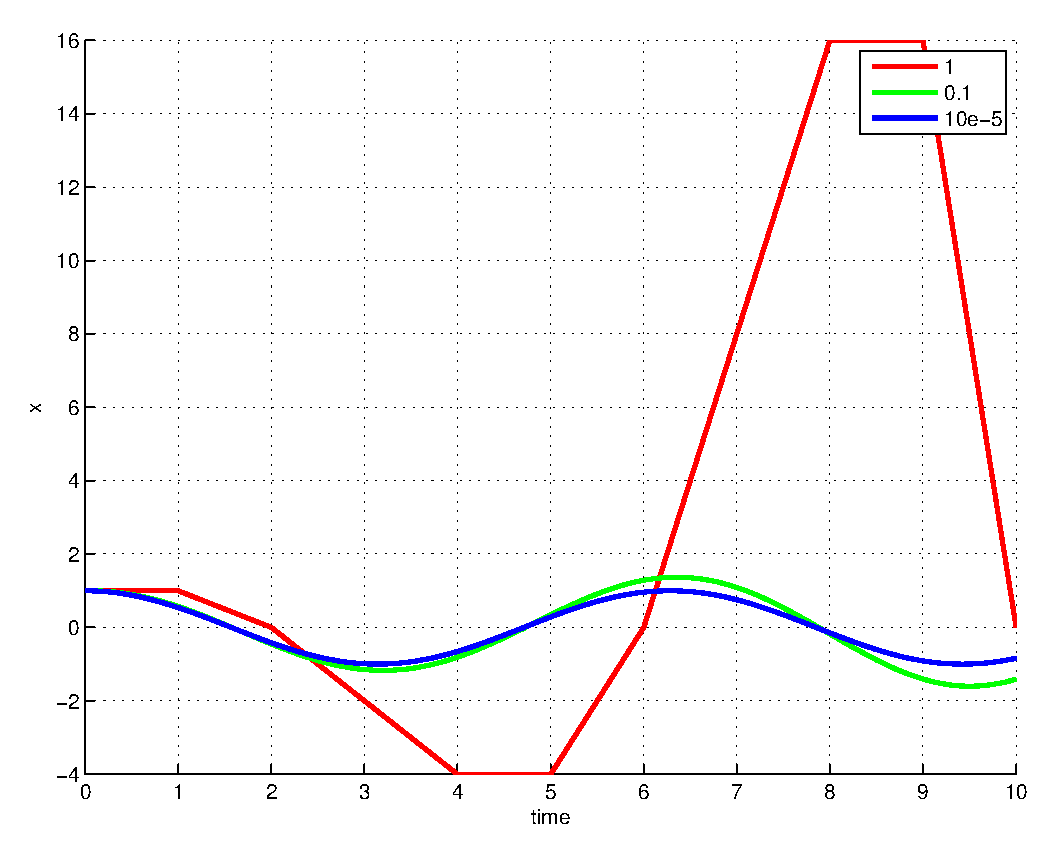
\includegraphics[width=4.5in]{exercise1c.eps}

The numerical solutions looks similar to the analytical one in case of small step sizes. If the step size parameter is to high, the sampling is less.

\item Simulation of a Hodgkin-Huxley neuron with forward Euler:
\begin{tiny}
\begin{lstlisting}
close all
clear all
clc

% Hodgkin Huxley simulation

%%%%%%%%%%%%%%%%%%%%%%%%%%%%%%%%%%%%%%%%%%%%%
%% I. Parameter %%%%%%%%%%%%%%%%%%%%%%%%%%%%%
simulationTime = 200; %in milliseconds
deltaT=.01;
t=0:deltaT:simulationTime;


%%%%%%%%%%%%%%%%%%%%%%%%%%%%%%%%%%%%%%%%%%%%
%% II. Specification of external current %%%
I(1:1000) = 0; I(1001:2000) = 3; I(2001:numel(t)) = 0;

% in order to plot result of exercise 2.4 uncomment the following lines
%% rheobase
I = 0.15*t;

%% inhibitory rebound
I(1:5000) = 0; I(5001:10000) = -3; I(10001:numel(t)) = 0;

%% resonant spiking
I(1:5000) = 0; I(5001:6000) = 2.05; I(6001:7000) = 0; I(7001:8000) = 2.05; I(8001:9000) = 0;
I(9001:10000) = 2.05; I(10001:11000) = 0; I(11001:12000) = 2.05; I(12001:numel(t)) = 0;

%%%%%%%%%%%%%%%%%%%%%%%%%%%%%%%%%%%%%%%%%%%%
%% III. Model parameter %%%%%%%%%%%%%%%%%%%%
gbar_K=36; gbar_Na=120; g_L=.3; % concutivities
E_K = -12; E_Na=115; E_L=10.6; % Nernst potentials
C=1; % membrane capacitance

%%%%%%%%%%%%%%%%%%%%%%%%%%%%%%%%%%%%%%%%%%%%
%% IV. Initial values for Euler %%%%%%%%%%%%
V=0; %Baseline voltage
alpha_n = ( (0.1-0.01*V) / (exp(1  -0.1*V)-1) ); % alpha n gate
alpha_m = ( (2.5- 0.1*V) / (exp(2.5-0.1*V)-1) ); % alpha m gate
alpha_h = 0.07*             exp(-V/20); % alpha h gate
beta_n  = 0.125*            exp(-V/80); % beta n gate
beta_m  = 4*                exp(-V/18); % beta m gate
beta_h  = 1              / (exp(3-0.1*V)+1); % beta h gate

n(1) = alpha_n/(alpha_n+beta_n); % channel activation n gate
m(1) = alpha_m/(alpha_m+beta_m); % channel activation m gate
h(1) = alpha_h/(alpha_h+beta_h); % channel activation h gate

for i=1:numel(t)-1 %Compute coefficients, currents, and derivates at each time step
    
    %%%%%%%%%%%%%%%%%%%%%%%%%%%%%%%%%%%%%%%%%%%%
    %% V. Calculate coefficients %%%%%%%%%%%%%%%
    %Equations here are same as above, just calculating at each time step
    alpha_n(i) = ( (0.1-0.01*V(i)) / (exp(1  -0.1*V(i))-1) );
    alpha_m(i) = ( (2.5- 0.1*V(i)) / (exp(2.5-0.1*V(i))-1) );
    alpha_h(i) = .07*                 exp(-V(i)/20);
    beta_n(i)  = 0.125*               exp(-V(i)/80);
    beta_m(i)  = 4*                   exp(-V(i)/18);
    beta_h(i)  = 1                 / (exp(3-0.1*V(i))+1);
    
    %%%%%%%%%%%%%%%%%%%%%%%%%%%%%%%%%%%%%%%%%%%%
    %% VI. Calculate currents %%%%%%%%%%%%%%%%%%
    I_Na = (m(i)^3) * gbar_Na * h(i) * (V(i)-E_Na); %Equations 3 and 14
    I_K = (n(i)^4) * gbar_K * (V(i)-E_K); %Equations 4 and 6
    I_L = g_L *(V(i)-E_L); %Equation 5
    I_ion = I(i) - I_K - I_Na - I_L; 
    
    %%%%%%%%%%%%%%%%%%%%%%%%%%%%%%%%%%%%%%%%%%%%
    %% VII. Calculate derivatives %%%%%%%%%%%%%%
    V(i+1) = V(i) + deltaT*I_ion/C;
    n(i+1) = n(i) + deltaT*(alpha_n(i) *(1-n(i)) - beta_n(i) * n(i)); %Equation 7
    m(i+1) = m(i) + deltaT*(alpha_m(i) *(1-m(i)) - beta_m(i) * m(i)); %Equation 15
    h(i+1) = h(i) + deltaT*(alpha_h(i) *(1-h(i)) - beta_h(i) * h(i)); %Equation 16

end

V = V-65; %Set resting potential to -65mv to deal with shift

%%%%%%%%%%%%%%%%%%%%%%%%%%%%%%%%%%%%%%%%%%%%
%% VIII. Plot voltage %%%%%%%%%%%%%%%%%%%%%%
figure
subplot(311)
grid on
hold on
plot(t,I,'r','lineWidth',3)
legend('current')
ylabel('current (mA)')
xlabel('time (ms)')
title('Stimulus current')
subplot(312)
plot(t,V,'LineWidth',3)
grid on
hold on
legend({'voltage'})
ylabel('Voltage (mv)')
xlabel('time (ms)')
title('Membrane potential')
subplot(313)
p1 = plot(t,gbar_K*n.^4,'LineWidth',2); % plot potassium conductance
grid on
hold on
p2 = plot(t,gbar_Na*(m.^3).*h,'r','LineWidth',2); % plot sodium conductance
legend([p1, p2], 'Conductance for Potassium', 'Conductance for Sodium')
ylabel('Conductance')
xlabel('time (ms)')
title('Conductance for Potassium and Sodium Ions')
\end{lstlisting}
\end{tiny}
\end{enumerate}
Use a step function as input:

  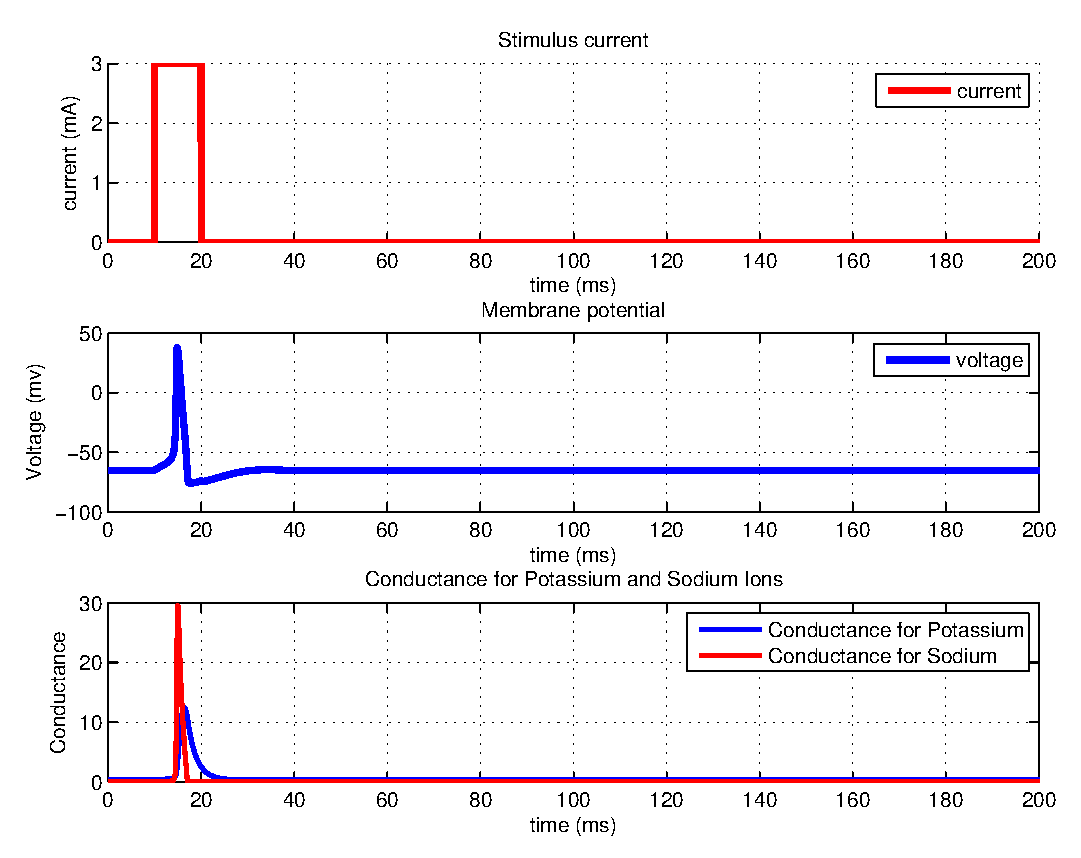
\includegraphics[width=5in]{exercise1d.eps}

\end{exercise}

\begin{exercise}{2.2}
Channel activation functions \\
\renewcommand{\labelenumi}{\alph{enumi})}
\begin{enumerate}
\item Use linear increasing current as input:

  \includegraphics[width=5in]{rheobase.eps}

\item Use step function with negatvie amplitude as input:

  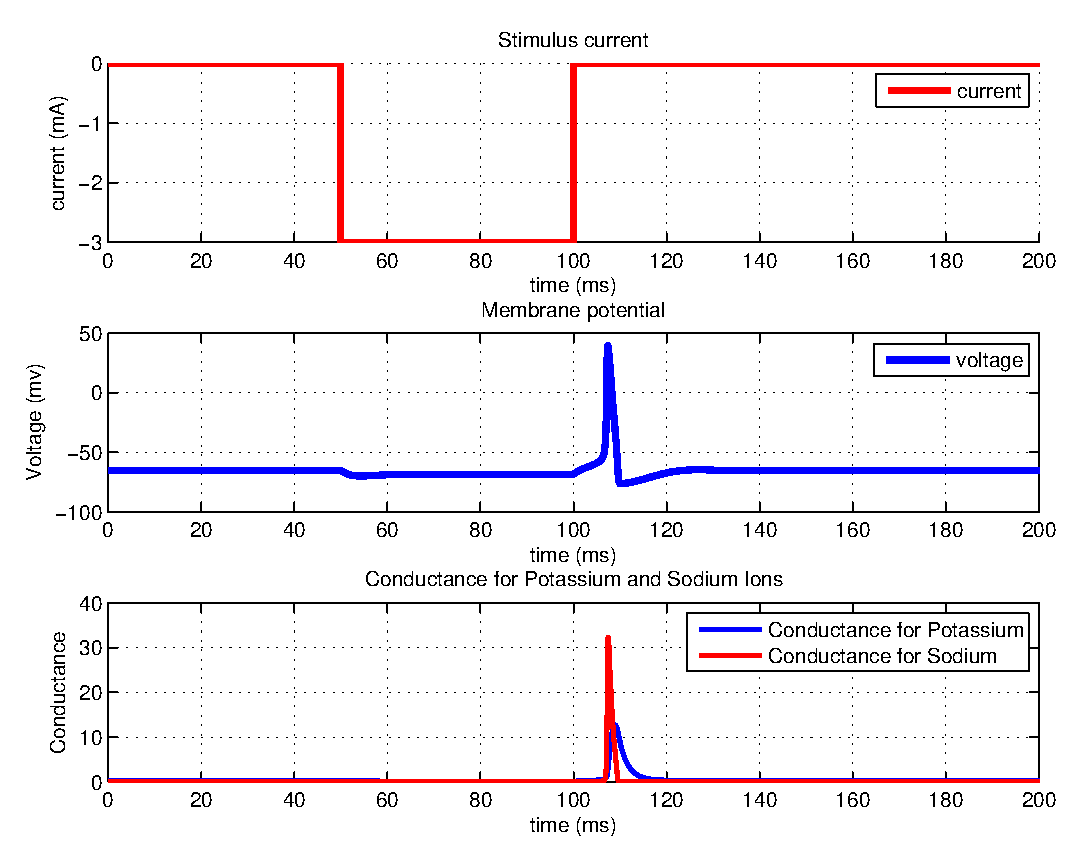
\includegraphics[width=5in]{inhrebound.eps}

\item Use equally spaced pulse sequence:

  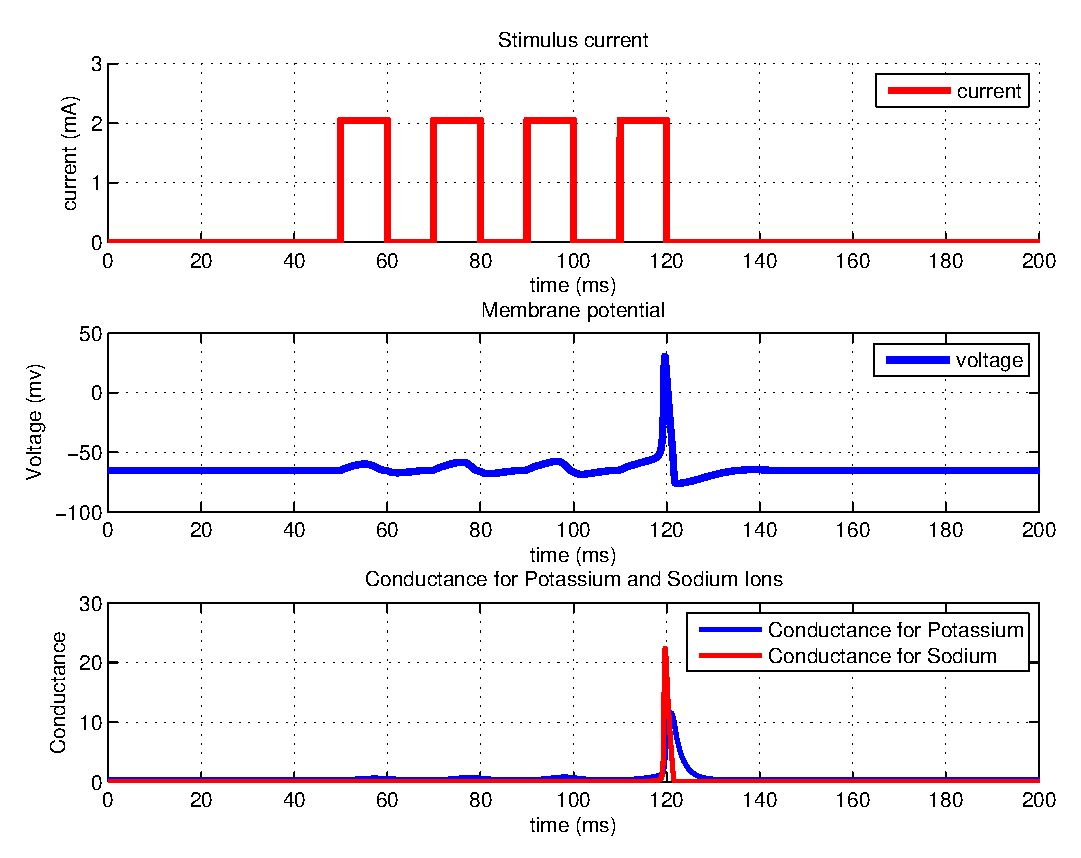
\includegraphics[width=5in]{resspiking.eps}

\end{enumerate}

\end{exercise}
 
\end{document}